\documentclass{report}

\usepackage[english, russian]{babel}
\usepackage{geometry}
\usepackage{listings}
\usepackage[T2A]{fontenc}
\usepackage[14pt]{extsizes}
\usepackage{color}
\usepackage[table,xcdraw]{xcolor}
\usepackage{multirow}
\usepackage{graphicx}
\usepackage[titles]{tocloft}
\usepackage[hyphens]{url}


\geometry{a4paper,top=2cm,bottom=2cm,left=2cm,right=1.5cm}
\setlength{\parskip}{0.5cm}
\setcounter{tocdepth}{4}
\setcounter{secnumdepth}{4}
\sloppy

\lstset
{
    language=C++,
    basicstyle=\footnotesize,
    numbers=left,
    numberstyle=\tiny,
    numberfirstline=true,
    numbersep=5pt,
    keywordstyle=\color{blue}\bfseries,
    commentstyle=\color{green},
    stringstyle=\color{red},
    showspaces=false,
    showstringspaces=false,
    captionpos=t,
    breaklines=true,
    breakatwhitespace=false,
    extendedchars=true,
    frame=tb,
    title=\lstname,
}


\begin{document}
    \begin{titlepage}

        \begin{center}
            \textbf{Федеральное государственное автономное образовательное учреждение высшего образования} \\
            "Национальный исследовательский Нижегородский государственный университет им. Н.И. Лобачевского" (ННГУ) \\
            \textbf{Институт информационных технологий, математики и механики}

            \vspace{\fill}

            \textbf{\LargeОтчет по лабораторной работе \\}
            \textbf{\large\\ «Поразрядная сортировка для вещественных чисел (тип double) с простым слиянием»}

            \vspace{\fill}

            \hfill\parbox{8cm}
            {
                \hspace*{5cm}\hspace*{-5cm}\textbf{Выполнил:} \\ Студент группы 381708-1 \\ Савкин Юрий Борисович \\ \\ \\
                \hspace*{5cm}\hspace*{-5cm}\textbf{Проверил:}\\ Доцент кафедры МОСТ, \\ кандидат технических наук \\ Сысоев А. В.
            }

            \vspace{\fill}

            Нижний Новгород \\ 2020 г.
        \end{center}

    \end{titlepage}


    \setcounter{page}{2}
    \setlength{\cftsecindent}{0em}
    \setlength{\cftsubsecindent}{1.25em}
    \setlength{\cftsubsubsecindent}{2.5em}
    \setlength{\cftsubsubsecnumwidth}{1.25em}
    \tableofcontents


    \newpage
    \section*{1. Введение}
    \addcontentsline{toc}{section}{1. Введение}
    \par Поразрядная сортировка - один из алгоритмов сортировки, работающих за линейное время.
         Этот алгоритм можно применить ко всем объектам, которые можно поделить на условные ``разряды''. В частности действительные числа типа \verb|double| языка C++.
    \par Существует два варианта поразрядной сортировки: LSD (least significant digit) и MSD (most significant digit).
         В первом случае сортировка начинается с младших разрядов, а во втором со старших. В данной работе будет рассматриваться только алгоритм LSD.
    \par Целью данной работы является изучение и реализация алгоритма поразрядной сортировки для вещественных чисел.
         Также исследуется возможность распараллеливания этого алгоритма с помощью различных технологий.


    \newpage
    \section*{2. Постановка задачи}
    \addcontentsline{toc}{section}{2. Постановка задачи}

    \par В ходе данной лабораторной работы необходимо:
    \begin{itemize}
        \item изучить алгоритм поразрядной сортировки
        \item написать последовательную версию алгоритма сортировки
        \item написать параллельные реализации алгоритма сортировки с помощью технологий OpenMP, TBB и потоков стандартной библиотеки языка C++ (\verb|std::thread|)
        \item проверить корректность работы реализованных алгоритмов
        \item сравнить результаты и сделать выводы об эффективности написанных реализаций
    \end{itemize}


    \newpage
    \section*{3. Описание алгоритма}
    \addcontentsline{toc}{section}{3. Описание алгоритма}

    \par В начале поразрядной сортировки сортируемые объекты делятся на разряды. Для типа double разрядом могут служить отдельные байты этого числа.
         Такое разбиение позволит корректно сортировать действительные числа из-за особенностей их представления в памяти.
         Бит числа тем больше вкладывает в значение числа, чем старше его позиция.
         Единственное исключение -- последний байт необходимо сортировать по другим условиям из-за того что старший бит действительного числа, отвечающий за знак, для отрицательных значений числа устанавливается в 1, а для положительных в 0.
    \begin{figure}[htbp]
        \centering
        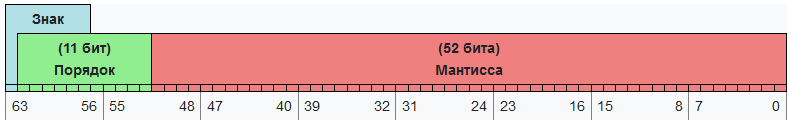
\includegraphics[width=0.9\textwidth]{../../../../modules/reports/savkin_y_radix_sort_simple_merge_double/double_precision.png}
        \caption{Представление типа double в памяти}
    \end{figure}
    \par Сравнение производится поразрядно начиная от младших разрядов. Элементы группируются по значениям текущего разряда.
         Затем элементы исходного массива перезаписываются в него в порядке, определённым значением их группы.
         Затем аналогичная операция повторяется для следующего разряда и так до предпоследнего.
         Алгоритм на последнем разряде отличается тем, что порядок групп для разрядов со старшими битами 1 и 0 формируется отдельно и перезаписывание в исходный массив начинается с групп со старшим разрядом 1.


    \newpage
    \section*{4. Схема распараллеливания}
    \addcontentsline{toc}{section}{4. Схема распараллеливания}
    \par Для реализации параллельных версий алгоритма поразрядной сортировки в начале исходный массив разбивается на части (по количеству потоков).
         Затем каждый поток сортирует свою часть массива с помощью алгоритма поразрядной сортировки.
         После этого происходит слияние отсортированных частей в исходный массив. В схеме простого слияния слиянием двух частей массива занимается 1 поток.


    \newpage
    \section*{5. Программная реализация}
    \par В данном разделе содержится краткое описание схем параллельного выполнения. Полный код находится в приложении.
    \par В качестве общей идеи параллельной реализации используется разбиение алгоритма на задачи. Для этого был создан ряд классов функторов для поразрядной сортировки части массива и для слияния 2 частей массива.
         Каждой программе можно указать на какое число частей нужно разбивать исходный массив, что в частности указывает число создающихся задач.
         Наибольшей эффективности можно добиться если число частей будет равно числу потоков.

    \addcontentsline{toc}{section}{5. Программная реализация}

    \subsection*{5.1. Особенности реализации с использованием OpenMP}
    \addcontentsline{toc}{subsection}{5.1. Особенности реализации с использованием OpenMP}
    \par Для каждой задачи создаётся список из зависящих от неё задач, и устанавливается число зависимостей (указывает у какого количества задач текущая находится в списке).
         В начале работы создаётся определённое число задач с поразрядной сортировкой и слиянием, а также устанавливаются зависимости между ними.
         Кроме того создаётся очередь задач, в которую попадают задачи, число зависимостей которых равно 0.
         Затем внутри параллельного блока потоки синхронизировано обращаются к очереди задач и берут себе задачу на исполнение.
         После исполнения задачи, для всех задач, зависящих от неё, уменьшается число зависимостей на 1. Задачи, у которых это число становится нулём добавляются в очередь.
         Этот процесс завершится, когда все задачи выполнятся.
         Для организации параллельного блока исполнения использовалась директива препроцессора \verb|#pragma omp parallel|.
         Для синхронизации доступа к очереди задач используется объект \verb|omp_lock_t| и функции \verb|omp_init_lock|, \verb|omp_set_lock|, \verb|omp_unset_lock| и \verb|omp_destroy_lock|.

    \subsection*{5.2. Особенности реализации с использованием TBB}
    \addcontentsline{toc}{subsection}{5.2. Особенности реализации с использованием TBB}
    \par Все функторы наследуются от класса \verb|tbb::task|. В начале работы создаётся главная задача с помощью \verb|new(tbb::task::allocateroot())| и ставится на исполнение с помощью функции \verb|tbb::task::spawn_root_and_wait|.
         В каждой задаче динамически создаются дочерние задачи с помощью \verb|new(allocate_child())| и затем рекурсивно ставятся на исполнение с помощью функции \verb|spawn_and_wait_for_all|.
         Задачи распределяются по потокам средствами TBB.

    \subsection*{5.3. Особенности реализации с использованием std::thread}
    \addcontentsline{toc}{subsection}{5.3. Особенности реализации с использованием std::thread}
    \par Схема создания задач и установки зависимостей между ними совпадает с таковой у реализации с использованием OpenMP.
         Отличие реализаций заключается только в том, какие функции и объекты используются в параллельном блоке.
         Для создания потоков используются объекты класса \verb|std::thread|. В их конструктор передаётся функция с доступом к очереди задач. В этой функции и находится параллельный блок.
         Для синхронизации доступа к очереди задач используется объект \verb|std::mutex|.
         Для того чтобы потоки не расходовали время процессора, если для них не нашлось доступной задачи используется функция \verb|std::this_thread::yield|.
         После исполнения параллельного блока вызывается функция ожидания завершения созданных потоков \verb|join()|.


    \newpage
    \section*{6. Результаты экспериментов и описание подтверждения корректности}
    \addcontentsline{toc}{section}{6. Результаты экспериментов и описание подтверждения корректности}
    \par Для подтверждения работоспособности и корректности работы написанных реализаций был создан ряд тестов. Полный код тестов представлен в приложении.
         Помимо этого был проведён ряд вычислительных экспериментов, для демонстрации эффективности параллельных реализаций.
    \par Конфигурация системы, на которой проводились эксперименты:
    \begin{itemize}
        \item Процессор: amd ryzen 5 2600 six-core processor 3.40 ghz (6 ядер / 12 потоков)
        \item Оперативная память: 16 GB
        \item Операционная система: Windows 7
        \item Компилятор: Visual C++
    \end{itemize}

    \par Эксперимент состоял из сортировки произвольного массива размером 50000000 элементов, при использовании различного числа потоков.
         На графике представлено время работы с использованием OpenMP, TBB и std::thread.
    \begin{figure}[htbp]
        \centering
        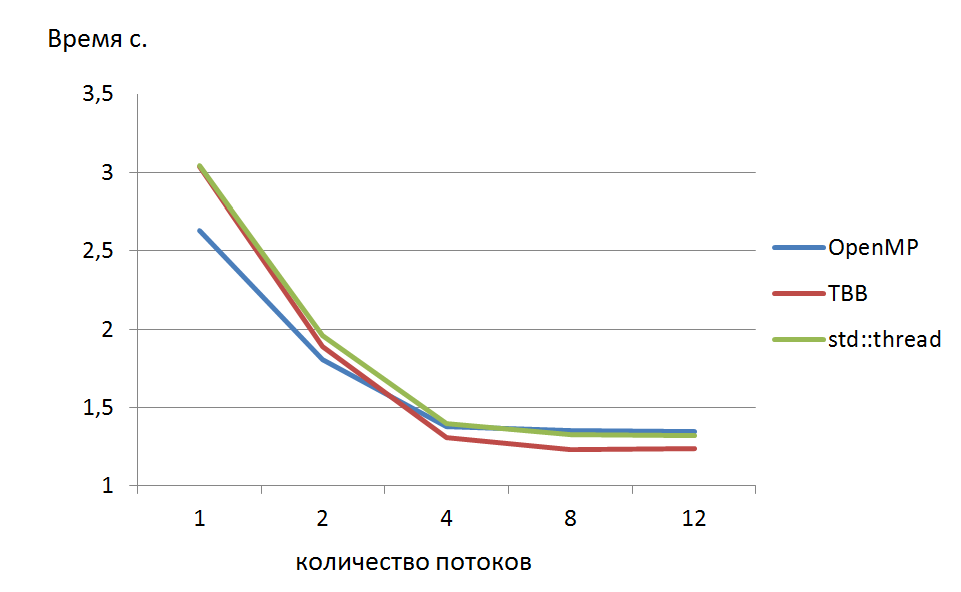
\includegraphics[width=0.99\textwidth]{../../../../modules/reports/savkin_y_radix_sort_simple_merge_double/diagram1.png}
        \caption{Время работы сортировок.}
    \end{figure}

    \par на следующем графике представлено ускорение по отношению к выполнению на 1 процессе.
    \begin{figure}[htbp]
        \centering
        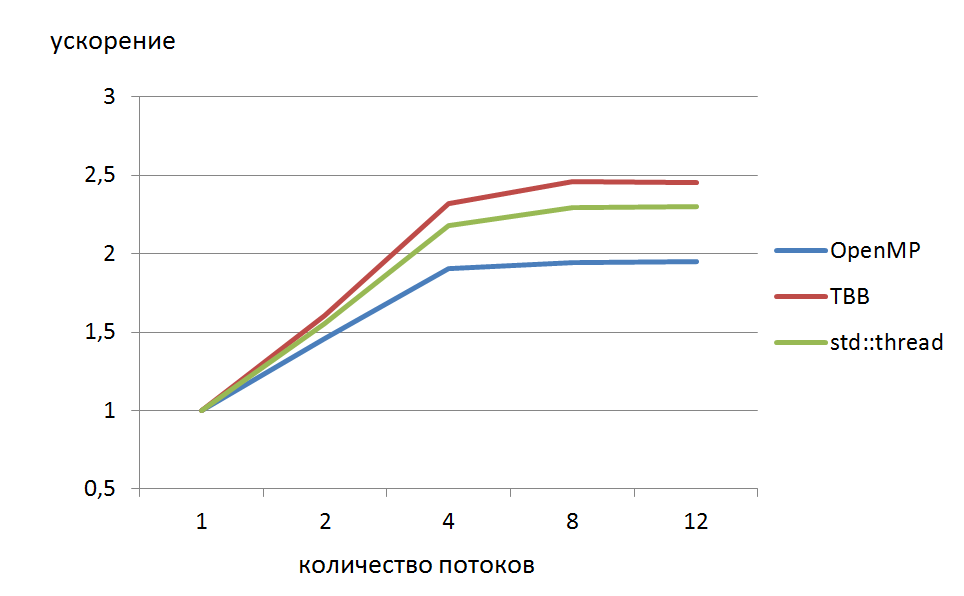
\includegraphics[width=0.99\textwidth]{../../../../modules/reports/savkin_y_radix_sort_simple_merge_double/diagram2.png}
        \caption{Время работы сортировок.}
    \end{figure}

    \begin{table}[htbp]
        \centering
        \begin{tabular}{|
            >{\columncolor[HTML]{EFEFEF}}c |c|c|c|}
            \hline
            \cellcolor[HTML]{68CBD0}                                     & \multicolumn{3}{c|}{\cellcolor[HTML]{68CBD0}время работы с.}                                       \\ \cline{2-4}
            \multirow{-2}{*}{\cellcolor[HTML]{68CBD0}количество потоков} & \cellcolor[HTML]{68CBD0}OpenMP & \cellcolor[HTML]{68CBD0}TBB & \cellcolor[HTML]{68CBD0}std::thread \\ \hline
            1                                                            & 2,63106                        & 3,03474                     & 3,0428                              \\ \hline
            2                                                            & 1,80745                        & 1,8875                      & 1,95614                             \\ \hline
            4                                                            & 1,37996                        & 1,3068                      & 1,39518                             \\ \hline
            8                                                            & 1,35172                        & 1,23227                     & 1,32603                             \\ \hline
            12                                                           & 1,34921                        & 1,23803                     & 1,32283                             \\ \hline
        \end{tabular}
        \caption{Результаты экспериментов.}
    \end{table}


    \newpage
    \section*{7. Заключение}
    \addcontentsline{toc}{section}{7. Заключение}

    \par В результате выполнения данной работы был изучен алгоритм поразрядной сортировки и возможность его распараллеливания путём разбиения исходного массива на части с последующим простым слиянием.
         Были реализованы 4 версии этого алгоритма: последовательная, с использованием OpenMP, с использованием TBB и с использованием потоков стандартной библиотеки языка C++ (\verb|std::thread|).
         Реализации показали свою работоспособность и эффективность. Скорость работы параллельных версий реализации увеличивалась при увеличении числа потоков.
         В целом все параллельные реализации показывают примерно одинаковое время работы и ускорение.


    \newpage
    \section*{8. Список литературы}
    \addcontentsline{toc}{section}{8. Список литературы}
    \begin{enumerate}
        \item Сысоев А.В., Мееров И.Б., Сиднев А.А. Средства разработки параллельных программ для систем с общей памятью. Библиотека Intel Threading Building Blocks. Учебно-методические материалы по программе повышения квалификации «Технологии высокопроизводительных вычислений для обеспечения учебного процесса и научных исследований». Нижний Новгород, 2007, 86 с.
        \item Guide into OpenMP: Easy multithreading programming for C++. URL: \url{https://bisqwit.iki.fi/story/howto/openmp/}
        \item Intel Threading Building Blocks User Guide. URL: \url{https://www.threadingbuildingblocks.org/docs/help/tbb_userguide/parallel_for.html}
    \end{enumerate}

    \newpage
    \section*{9. Приложение}
    \addcontentsline{toc}{section}{9. Приложение}

    \subsection*{Исходный код}
    \addcontentsline{toc}{subsection}{Исходный код}

    \subsubsection*{Лабораторная работа №1. Последовательная версия}
    \addcontentsline{toc}{subsubsection}{Лабораторная работа №1. Последовательная версия}
    \lstinputlisting[language=C++, caption=Последовательная версия. Заголовочный файл]{../../../../modules/task_1/savkin_y_radix_sort_simple_merge_double/radix_sort_simple_merge_double.h}
    \lstinputlisting[language=C++, caption=Последовательная версия. Файл с реализацией]{../../../../modules/task_1/savkin_y_radix_sort_simple_merge_double/radix_sort_simple_merge_double.cpp}
    \lstinputlisting[language=C++, caption=Последовательная версия. Файл с тестами]{../../../../modules/task_1/savkin_y_radix_sort_simple_merge_double/main.cpp}

    \newpage
    \subsubsection*{Лабораторная работа №2. Параллельная версия с использованием OpenMP}
    \addcontentsline{toc}{subsubsection}{Лабораторная работа №2. Параллельная версия с использованием OpenMP}
    \lstinputlisting[language=C++, caption=Параллельная версия с использованием OpenMP. Заголовочный файл]{../../../../modules/task_2/savkin_y_radix_sort_simple_merge_double/radix_sort_simple_merge_double.h}
    \lstinputlisting[language=C++, caption=Параллельная версия с использованием OpenMP. Файл с реализацией]{../../../../modules/task_2/savkin_y_radix_sort_simple_merge_double/radix_sort_simple_merge_double.cpp}
    \lstinputlisting[language=C++, caption=Параллельная версия с использованием OpenMP. Файл с тестами]{../../../../modules/task_2/savkin_y_radix_sort_simple_merge_double/main.cpp}

    \newpage
    \subsubsection*{Лабораторная работа №3. Параллельная версия с использованием TBB}
    \addcontentsline{toc}{subsubsection}{Лабораторная работа №3. Параллельная версия с использованием TBB}
    \lstinputlisting[language=C++, caption=Параллельная версия с использованием TBB. Заголовочный файл]{../../../../modules/task_3/savkin_y_radix_sort_simple_merge_double/radix_sort_simple_merge_double.h}
    \lstinputlisting[language=C++, caption=Параллельная версия с использованием TBB. Файл с реализацией]{../../../../modules/task_3/savkin_y_radix_sort_simple_merge_double/radix_sort_simple_merge_double.cpp}
    \lstinputlisting[language=C++, caption=Параллельная версия с использованием TBB. Файл с тестами]{../../../../modules/task_3/savkin_y_radix_sort_simple_merge_double/main.cpp}

    \newpage
    \subsubsection*{Лабораторная работа №4. Параллельная версия с использованием std::thread}
    \addcontentsline{toc}{subsubsection}{Лабораторная работа №4. Параллельная версия с использованием std::thread}
    \lstinputlisting[language=C++, caption=Параллельная версия с использованием std::thread. Заголовочный файл]{../../../../modules/task_4/savkin_y_radix_sort_simple_merge_double/radix_sort_simple_merge_double.h}
    \lstinputlisting[language=C++, caption=Параллельная версия с использованием std::thread. Файл с реализацией]{../../../../modules/task_4/savkin_y_radix_sort_simple_merge_double/radix_sort_simple_merge_double.cpp}
    \lstinputlisting[language=C++, caption=Параллельная версия с использованием std::thread. Файл с тестами]{../../../../modules/task_4/savkin_y_radix_sort_simple_merge_double/main.cpp}

\end{document}